\chapter{线程}

\section{线程基础知识}

\subsection{线程状态}

JVM线程的状态定义在Thread.State枚举中。包括:

\begin{itemize}
    \item   NEW 
    \item   RUNNABLE 
    \item   BLOCKED 
    \item   WAITING 
    \item   TIMED\_WAITING
    \item   TERMINATED
\end{itemize}


\begin{figure}[H]
    \centering
    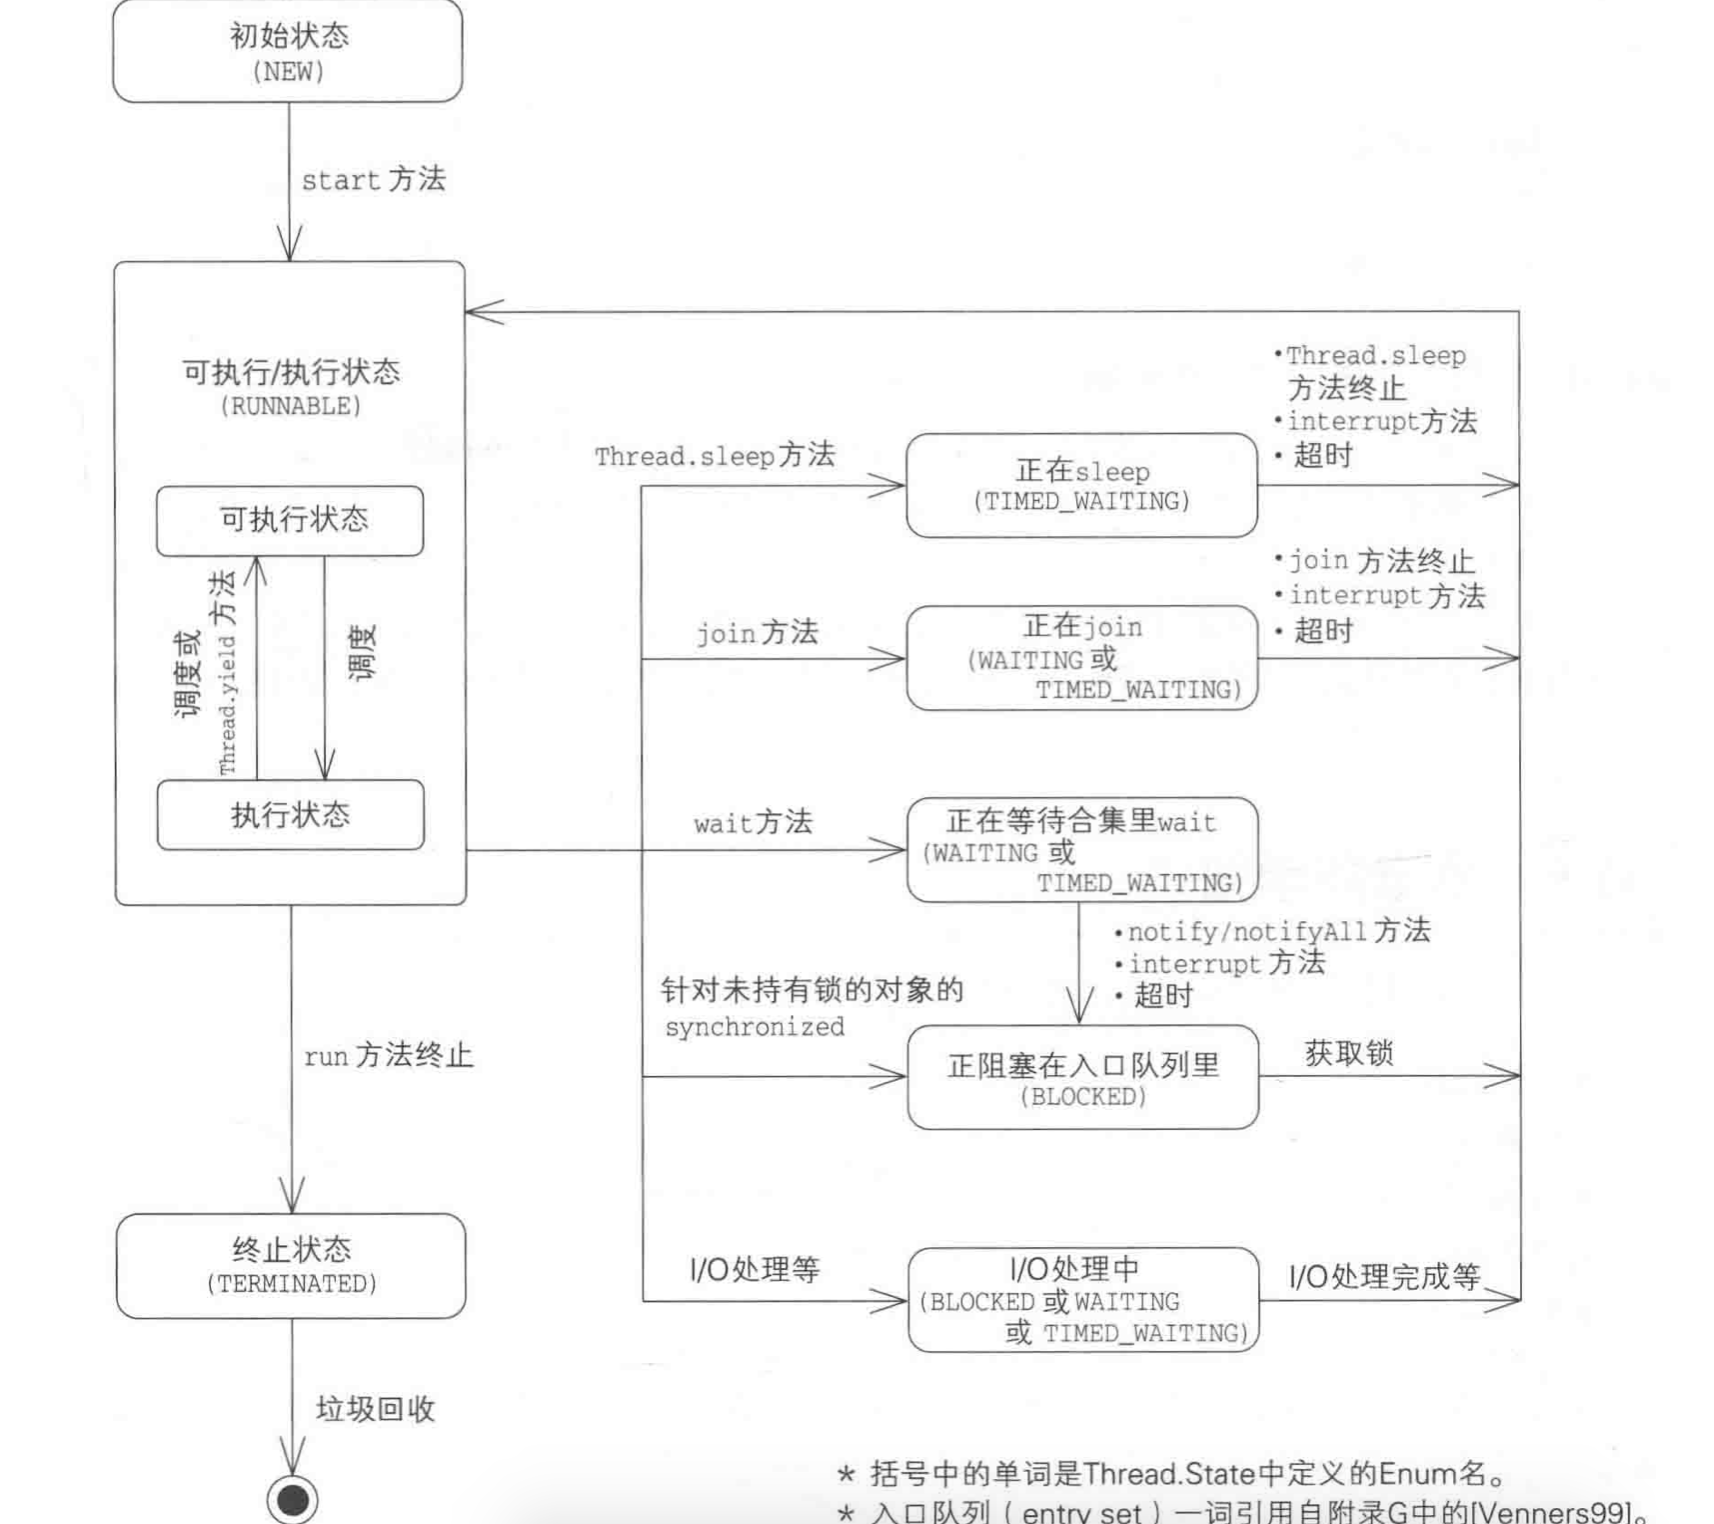
\includegraphics[width=1\textwidth]{thread/thread_states.png}
    \caption{线程状态迁移图(摘自《图解Java多线程设计模式》)}
\end{figure}

下面为State枚举


\begin{lstlisting}[language=java]

public enum State {
        /**
         * 尚未启动的线程的线程状态
         */
        NEW,

        /**
         * 可运行线程的线程状态。 处于可运行状态的线程正在Java虚拟机中执行,
         * 但是它可能正在等待来自操作系统(例如处理器)的其他资源。
         */
        RUNNABLE,

        /**
         * 线程的阻塞状态,等待监视器锁定。
         * 处于阻塞状态的线程正在等待一个监视器锁进入一个同步块/方法,
         * 或者在调用Object.wait()后重新进入一个同步块/方法。
         */
        BLOCKED,

        /**
         * 等待线程状态
         * 一个线程由于调用下列方法之一而处于等待状态:
         * 
         *   Object.wait() 未超时
         *   Thread.join() 未超时
         *   LockSupport.park()
         * 
         * <p>处于等待状态的线程正在等待另一个线程执行特定的操作。
         * 例如: 一个线程在一个对象上已经调用了 Object.wait() ,并正在等待在另一个线程在另一对象上调用
         * Object.notify() or Object.notifyAll()。
         * 调用 thread.join() 的线程正在等待指定的线程终止。
         */
        WAITING,

        /**
         * 具有指定等待时间的等待线程的线程状态。
         * 线程处于定时等待状态,因为调用以下方法之一与指定的正等待时间:
         * 
         *   Thread.sleep()
         *   Object.wait(long)带超时参数
         *   Thread.join(long)带超时参数
         *   LockSupport.parkNanos
         *   LockSupport.parkUntil
         * 
         */
        TIMED_WAITING,

        /**
         * 终止状态。线程已经完成执行。
         */
        TERMINATED;
    }

\end{lstlisting}

\subsection{常用函数}




\section{Synchronized}



